\section{Exempel}
Följande exempel är från boken Numerical Optimization av Jorge Nocedal och Stephen J. Wright släppt 1999 och är exempel 16.3 på sida 462.
\begin{figure}[h!]
  \centering
    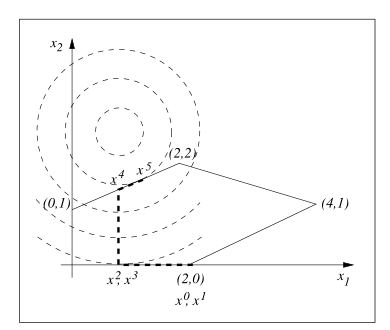
\includegraphics[width=0.5\textwidth]{grafik/exempel.png}
      \caption{Visualisering av problemet.}
\end{figure}

\begin{equation*}
\begin{aligned}
& \underset{x}{\text{minimize}}\
  q(x)=  (x_1-1)^2+(x_2-2.5)^2\\
 \text{subject to}\
 & x_1-2x_2+2 \geq0  \\
 -& x_1-2x_2+6 \geq0  \\
 & x_1+2x_2+2 \geq0  \\
 & x_1\geq0  \\
 & x_2\geq0  \\
 & z \in \mathbb{R}^N 
\end{aligned}
\end{equation*}
\captionof{figure}{Problembeskrivning}

Problemet kan skrivas om för att göra det enklare att beskriva det på matrisform:
\begin{equation*}
\begin{aligned}
& \underset{x}{\text{minimize}}\
  q(x)=  x_1^2+1^2-2x_1+x_2^2 +2.5^2-5x_ 2\\
 \text{subject to}\
 & x_1-2x_2 \geq-2  \\
 -& x_1-2x_2 \geq-6  \\
 & x_1+2x_2 \geq-2  \\
 & x_1\geq0  \\
 & x_2\geq0  \\
 & z \in \mathbb{R}^N 
\end{aligned}
\end{equation*}
Målfunktionen kan nu delas in i konstanta delar som vi inte kan påverka, linjära delar och kvadratiska delar.
Dessa kan sedan användas för att beskriva problemet i matrisform.
 \[
 G=
\begin{pmatrix*}[r]
  2 & 0 \\
  0 & 2
\end{pmatrix*}
\]
 
  \[
 d=
\begin{pmatrix*}[r]
  -2  \\
  -5 
\end{pmatrix*}
\]

  \[
 A=
\begin{pmatrix*}[r]
  1 & -2  \\
  -1 & -2  \\
  -1 & 2  \\
  1 & 0  \\
 0 & 1  \\
\end{pmatrix*}
\]

  \[
 b=
\begin{pmatrix*}[r]
   -2  \\
   -6  \\
   -2  \\
   0  \\
 0   \\
\end{pmatrix*}
\]
G och d beskriver målfunktionen, A och b beskriver bivillkoren i följande uppställning:
  \[
 x=
\begin{pmatrix*}[r]
   x_1  \\
   x_2 
\end{pmatrix*}
\]
\newline
\begin{equation*}
\begin{aligned}
& \underset{x}{\text{minimize}}
& & \frac{1}{2} x^{T}Gx+d^{T}x \\
& \text{subject to}
& & Ax\geq b \\
& && x \in \mathbb{R}^N \\
& && A \in \mathbb{R}^{m*N}
\end{aligned}
\end{equation*}
\captionof{figure}{Nästan normalform}

\begin{equation*}
\begin{aligned}
& \underset{x}{\text{minimize}}
& & 
\frac{1}{2}\begin{pmatrix*}[r]
   x_1  & x_2 
\end{pmatrix*}
\begin{pmatrix*}[r]
  2 & 0 \\
  0 & 2
\end{pmatrix*}
\begin{pmatrix*}[r]
   x_1  \\
   x_2 
\end{pmatrix*}
+
\begin{pmatrix*}[r]
  -2  &
  -5 
\end{pmatrix*}
\begin{pmatrix*}[r]
   x_1  \\
   x_2 
\end{pmatrix*}= x_1^2+1^2-2x_1+x_2^2 +2.5^2-5x_ 2\\
& \text{subject to}
& & Ax =\begin{pmatrix*}[r]
  1 & -2  \\
  -1 & -2  \\
  -1 & 2  \\
  1 & 0  \\
 0 & 1  \\
\end{pmatrix*}
\begin{pmatrix*}[r]
   x_1  \\
   x_2 
\end{pmatrix*}
 \geq b= \begin{pmatrix*}[r]
   -2  \\
   -6  \\
   -2  \\
   0  \\
 0   \\
\end{pmatrix*}\\
& && x \in \mathbb{R}^N \\
& && A \in \mathbb{R}^{m*N}
\end{aligned}
\end{equation*}
Så matriserna beskriver problemet.

Det första problemet är att hitta en startpunkt där man kan börja söka efter lösning. Det enklaste är att sätta x lika med nollvektorn, dvs:
  \[
 x=
\begin{pmatrix*}[r]
   x_1  \\
   x_2 
\end{pmatrix*}
=
\begin{pmatrix*}[r]
   0  \\
   0 
\end{pmatrix*}
\]
Sedan testa om denna punkt uppfyller alla bivillkor. I detta fall så är denna punkt okey men skulle den inte vara okey så sätter man lika många bivillkor som man har variabler lika med istället för mindre/större än. Dvs i detta exempel har vi 2 variabler och om vi gör om de två första bivillkoren till lika med villkor så för vi ett lösbart system. 
\begin{equation*}
\begin{aligned}
 & x_1-2x_2+2 =0  \\
 -& x_1-2x_2+6 =0  \\
\end{aligned}
\end{equation*}
Sedan testar vi denna punkt mot alla bivillkor. Skulle detta vara en ej godkänd punkt så testar men en annan kombination av bivillkor tills man hittar en godkänd startpunkt. 

I boken valde de följande startpunkt:

  \[
 x^0=
\begin{pmatrix*}[r]
   x_1  \\
   x_2 
\end{pmatrix*}
=
\begin{pmatrix*}[r]
   2  \\
   0 
\end{pmatrix*}
\]
Om man sittar på bivillkoren så kan man se att i denna punkt är bivillkoren 3 och 5 aktiva. Det vill säga punkten ligger på bivillkorens linjer. Då kan vi säga att mängden aktiva bivillkor består av bivillkor 3 och 5 och skrivs på följande sätt:
\begin{equation*}
W_0=\{ 3,5 \}
\end{equation*}
Nu kan vi lösa subproblemet definierat under definitioner.
  \[
 p^0=
\begin{pmatrix*}[r]
   p_1  \\
   p_2 
\end{pmatrix*}
\]

\begin{equation*}
\begin{aligned}
& \underset{p}{\text{minimize}}
& & \frac{1}{2}
 \begin{pmatrix*}[r]
   p_1  \\
   p_2 
\end{pmatrix*}^
 {T}
 \begin{pmatrix*}[r]
  2 & 0 \\
  0 & 2
\end{pmatrix*}
  \begin{pmatrix*}[r]
   p_1  \\
   p_2 
\end{pmatrix*}
 +
 g
 _0^{T}
  \begin{pmatrix*}[r]
   p_1  \\
   p_2 
\end{pmatrix*} \\
& \text{subject to}
& & 
  \begin{pmatrix*}[r]
   -1  &
   2 
\end{pmatrix*} 
  \begin{pmatrix*}[r]
   p_1  \\
   p_2 
\end{pmatrix*} 
= 0  \\
& & & 
  \begin{pmatrix*}[r]
   0  &
   1 
\end{pmatrix*} 
  \begin{pmatrix*}[r]
   p_1  \\
   p_2 
\end{pmatrix*} 
= 0  \\
\end{aligned}
\end{equation*}
\newline
\newline
\begin{equation*}
\begin{aligned}
& g_0=Gx_0+d =
 \begin{pmatrix*}[r]
  2 & 0 \\
  0 & 2
\end{pmatrix*}*
\begin{pmatrix*}[r]
   2  \\
   0 
\end{pmatrix*}
+
\begin{pmatrix*}[r]
  -2  \\
  -5 
\end{pmatrix*}
=
\begin{pmatrix*}[r]
  2  \\
  -5 
\end{pmatrix*}
\end{aligned}
\end{equation*}
Detta ger:
\begin{equation*}
\begin{aligned}
& \underset{p}{\text{minimize}}
& & \frac{1}{2}
 \begin{pmatrix*}[r]
   p_1  \\
   p_2 
\end{pmatrix*}^
 {T}
 \begin{pmatrix*}[r]
  2 & 0 \\
  0 & 2
\end{pmatrix*}
  \begin{pmatrix*}[r]
   p_1  \\
   p_2 
\end{pmatrix*}
 +
  \begin{pmatrix*}[r]
   2  &
   -5
\end{pmatrix*} 
  \begin{pmatrix*}[r]
   p_1  \\
   p_2 
\end{pmatrix*} \\
& \text{subject to}
& & 
-p_1+2p_2
= 0  \\
& & & 
p_2
= 0  \\
\end{aligned}
\end{equation*}
vilket ger
\begin{equation*}
\begin{aligned}
 p_1=p_2=0
 \end{aligned}
\end{equation*}
Vi kan nu beräkna Lagrange multiplikatorerna för denna iteration:
\begin{equation*}
\begin{aligned}
\sum_{i\in \hat{W}}a_i\hat{\lambda_i}=g=G\hat{x}+d
\end{aligned}
\end{equation*}

\begin{equation*}
\begin{aligned}
  \begin{pmatrix*}[r]
   -1  \\
   2 
\end{pmatrix*} \hat{\lambda}_3+
  \begin{pmatrix*}[r]
   0  \\
    1
\end{pmatrix*} \hat{\lambda}_5=
  \begin{pmatrix*}[r]
   2  \\
    -5
\end{pmatrix*}
\end{aligned}
\end{equation*}

\begin{equation*}
\begin{aligned}
-\hat{\lambda}_3=2 \\
2\hat{\lambda}_3+\hat{\lambda}_5=-5
\end{aligned}
\end{equation*}
Vilket ger:
\begin{equation*}
\begin{aligned}
  \begin{pmatrix*}[r]
   \hat{\lambda}_3  &
    \hat{\lambda}_5
\end{pmatrix*}=
  \begin{pmatrix*}[r]
   -2  &
    -1
\end{pmatrix*}
\end{aligned}
\end{equation*}
Detta leder till att vi tar bort bivillkor 3 från mängden då den har mest negativ Lagrange multiplikator.

\begin{equation*}
\begin{aligned}
W_1=\{ 5 \}
\end{aligned}
\end{equation*}
Vi löser subproblemet:

\begin{equation*}
\begin{aligned}
& \underset{p}{\text{minimize}}
& & \frac{1}{2}
 \begin{pmatrix*}[r]
   p_1  \\
   p_2 
\end{pmatrix*}^
 {T}
 \begin{pmatrix*}[r]
  2 & 0 \\
  0 & 2
\end{pmatrix*}
  \begin{pmatrix*}[r]
   p_1  \\
   p_2 
\end{pmatrix*}
 +
  \begin{pmatrix*}[r]
   2  &
   -5
\end{pmatrix*} 
  \begin{pmatrix*}[r]
   p_1  \\
   p_2 
\end{pmatrix*} \\
& \text{subject to}
& & p_2= 0  \\
\end{aligned}
\end{equation*}


\begin{equation*}
\begin{aligned}
 \underset{p}{\text{minimize}} \ \
p_1^2+2p_1
\end{aligned}
\end{equation*}
derivering ger:
\begin{equation*}
\begin{aligned}
2*p_1+2
\end{aligned}
\end{equation*}
som är 0 då:
\begin{equation*}
\begin{aligned}
p_1=-1
\end{aligned}
\end{equation*}
Andraderivatan är positiv vilket ger att det är en minpunkt, lösning ges av:

\begin{equation*}
\begin{aligned}
  \begin{pmatrix*}[r]
   p_1  \\
   p_2
\end{pmatrix*} =
  \begin{pmatrix*}[r]
   -1  \\
   0
\end{pmatrix*}
=p^1
\end{aligned}
\end{equation*}

Nu vet vi vart vi står och i vilken riktining vi ska gå. Nu ska vi beräkna hur långt vi ska gå med hjälp av stegformulan under definitioner.
\begin{equation*}
\begin{aligned}
\frac{b_i-a_i^Tx_k}{a_i^Tp_k}
\end{aligned}
\end{equation*}
Beräknas för alla villkor som inte tillhör den aktiva mängden. För i=1:

\begin{equation*}
\begin{aligned}
\frac{-2-
  \begin{pmatrix*}[r]
   1  &
   -2
\end{pmatrix*}
  \begin{pmatrix*}[r]
   2  \\
   0
\end{pmatrix*}
}{
  \begin{pmatrix*}[r]
   1  &
   -2
\end{pmatrix*}
  \begin{pmatrix*}[r]
   -1  \\
   0
\end{pmatrix*}}=\frac{-4}{-1}=4
\end{aligned}
\end{equation*}
Vilket är större än 1 så nuvarande $\alpha$ är 1
För i=2:

\begin{equation*}
\begin{aligned}
\frac{-6-
  \begin{pmatrix*}[r]
   -1  &
   -2
\end{pmatrix*}
  \begin{pmatrix*}[r]
   2  \\
   0
\end{pmatrix*}
}{
  \begin{pmatrix*}[r]
   -1  &
   -2
\end{pmatrix*}
  \begin{pmatrix*}[r]
   -1  \\
   0
\end{pmatrix*}}=\frac{-4}{1}=-4
\end{aligned}
\end{equation*}
vilket är mindre än 1 men $a_i^Tp_k>0$ så $\alpha $ är fortfarande 1
För i=3:

\begin{equation*}
\begin{aligned}
\frac{-2-
  \begin{pmatrix*}[r]
   -1  &
   2
\end{pmatrix*}
  \begin{pmatrix*}[r]
   2  \\
   0
\end{pmatrix*}
}{
  \begin{pmatrix*}[r]
   -1  &
   2
\end{pmatrix*}
  \begin{pmatrix*}[r]
   -1  \\
   0
\end{pmatrix*}}=\frac{0}{1}=0
\end{aligned}
\end{equation*}
vilket är mindre än 1 men $a_i^Tp_k>0$ så $\alpha $ är fortfarande 1

För i=4:

\begin{equation*}
\begin{aligned}
\frac{0-
  \begin{pmatrix*}[r]
   1  &
   0
\end{pmatrix*}
  \begin{pmatrix*}[r]
   2  \\
   0
\end{pmatrix*}
}{
  \begin{pmatrix*}[r]
   1  &
   0
\end{pmatrix*}
  \begin{pmatrix*}[r]
   -1  \\
   0
\end{pmatrix*}}=\frac{-2}{-1}=2
\end{aligned}
\end{equation*}
vilket är större än 1 så $\alpha $ är fortfarande 1. Detta ger:

\begin{equation*}
\begin{aligned}
x^2=x^1+p^1\alpha
\end{aligned}
\end{equation*}

\begin{equation*}
\begin{aligned}
  \begin{pmatrix*}[r]
   x_1  \\
   x_2
\end{pmatrix*}=
  \begin{pmatrix*}[r]
   2  \\
   0
\end{pmatrix*}+
  \begin{pmatrix*}[r]
   -1  \\
   0
\end{pmatrix*}*1
\end{aligned}
\end{equation*}

vilket ger:

\begin{equation*}
\begin{aligned}
x^2=
  \begin{pmatrix*}[r]
   1  \\
   0
\end{pmatrix*}
\end{aligned}
\end{equation*}
Nu kan man titta vilka villkor som är aktiva i denna punkt och använda detta för att lösa subproblemet och forsätter iterera tills vi vår en lösning med p=0 och positiva lagrange multiplikatorer